
\documentclass[a4paper,12pt]{article}

\usepackage{amsmath}
\usepackage{amssymb}
\usepackage[english]{babel}
\usepackage[margin=1in]{geometry}
\usepackage{graphicx}
\usepackage{listings}

\lstset{tabsize=3, basicstyle=\ttfamily\small, commentstyle=\itshape\rmfamily, numbers=left, numberstyle=\tiny, language=java,moredelim=[il][\sffamily]{?},mathescape=true,showspaces=false,showstringspaces=false,columns=fullflexible,xleftmargin=5pt,escapeinside={(@}{@)}, morekeywords=[1]{let,if,then,else}}
\lstloadlanguages{Java, Haskell}

\newcommand{\kwa}[1]{\mathtt{#1}}
\newcommand{\kw}[1]{\mathtt{#1}~}

\begin{document}

\section{Dijkstra's Algorithm}

\noindent
The shortest path problem in a directed graph involves finding the path from $\kwa{src}$ to $\kwa{dest}$ whose weights on the edge are least. One such algorithm to do this is Dijkstra's algorithm. The idea is to begin looking at paths starting at $\kwa{src}$, keeping them in a fringe of ``candidate paths''. On each iteration, consider the shortest candidate path and add another edge to it. You repeat the process until you find the shortest candidate path ending at $\kwa{dest}$. Here is some pseudocode fro Dijkstra's algorithm, which will find the shortest path in a directed, weighted graph:

\begin{lstlisting}
Dijkstras(src, dest) {
   pq = $\varnothing$, visited = $\varnothing$
   pq.offer(<src, null, 0>)
   while (pq $\neq$ $\varnothing$) {
      <node, from, costSoFar> = pq.pop()
      if (node == dest) return the path
      if (node $\in$ visited) continue
      visited.add(node)
      for (neigh : node.neighbours()) {
         pq.offer(<neigh, node, costSoFar + weight(node, neigh)>)
      }
   }
   return null
}
\end{lstlisting}

\noindent
The fringe is a priority queue of triples $\kwa{<node, from, costSoFar>}$. A triple has greater priority if it has a lower $\kwa{costSoFar}$. For example, if the queue consisted of two triples, $\kwa{<A, B, 15>}$ and $\kwa{<C, D, 10>}$, then the second would be popped off the fringe first. 

The $\kwa{from}$ field is supposed to be a representation of the path taken so far, i.e. it is another triple. For brevity, we usually just refer to the from field by the last node on that path. When a triple $\kwa{<node, from, costSoFar>}$ is popped off the priority queue, we consider the path obtained by adding the edge from the node $\kwa{from}$ to the node $\kwa{node}$. That path could be extended by adding on any edge coming out of $\kwa{node}$, so lines 9-10 adds a bunch of candidate paths, one for each outgoing edge.

When a node $\kwa{n}$ has been visited, the path along which it is visited will be the shortest path from $\kwa{src}$ to $\kwa{n}$. Any path to $\kwa{dest}$ which goes through$ \kwa{n}$ must extend that path; therefore, nodes are visited exactly once. This is the purpose of the check on line 7.

If the node being visited is the goal node, we must reconstruct the path and return it. If the fringe becomes empty, meaning every path starting at $\kwa{src}$ has been considered, and $\kwa{dest}$ was never visited, then there is no path from $\kwa{src}$ to $\kwa{dest}$ --- line 13 returns $\kwa{null}$ in this situation.

Here is one representation of the triples that must be stored in the Fringe, in Java:

\begin{lstlisting}
class Triple implements Comparable<Triple> {
   private Triple from;
   private int costSoFar;
   private Node nodeToVisit;
   
   @Override
   public int compareTo(Job other) {
      ...
   }
}
\end{lstlisting}

\noindent
The priority queue must privilege triples according to their $\kwa{costSoFar}$ field (choosing the one with the lowest $\kwa{costSoFar}$), so we need to specify this in Java. One way is to have $\kwa{Triple}$ implement $\kwa{Comparable<Triple>}$, defining a ``natural ordering'' for the priority queue to use. Another is to define a $\kwa{Comparator}$ for comparing triples and pass this into the priority queue when it is instantiated.

If you represent triples like above, then when you pop a triple $\kwa{<dest, from, costSoFar>}$, you can reconstruct the path from $\kwa{src}$ to $\kwa{dest}$ by repeatedly following the $\kwa{from}$ field, gathering up the nodes in each triple, until you get to the initial triple $\kwa{<src, null, 0>}$. The path will be backwards, so you will have to reverse it.

Dijkstra's is a greedy algorithm, meaning you always choose the ``best looking'' candidate path (i.e. the one with the shortest $\kwa{costSoFar}$) on each iteration. In certain situations, this algorithm returns the shortest path, but in some cases it doesn't work:

\begin{enumerate}
	\item If $\kwa{src}$ and $\kwa{dest}$ are in different components of the graph, there is no shortest path (or indeed, any path) between them.
	\item If you permit repeated edges in your paths and there is a negative edge-weight cycle en route to $\kwa{dest}$ from $\kwa{src}$, no shortest path exists: any supposed ``shortest path'' can be made shorter by going around the loop again.
	\item If there are negative edge weights, the shortest path may not be found.
\end{enumerate}

\noindent
To illustrate why Dijkstra's may fail in the third situation, consider the below graph. The shortest path is A $\rightarrow$ B $\rightarrow$ D, but the ``shortest path'' returned by the algorithm is A $\rightarrow$ C $\rightarrow$ D. This is because Dijkstra's will greedily choose the best looking path at each stage, and the second path initially looks better, because there is a high cost associated with the edge $A \rightarrow B$ --- however, this high cost is later offset by the negative cost on B $\rightarrow C$. Dijkstra's greedy approach never considers it though.

~\\~\\
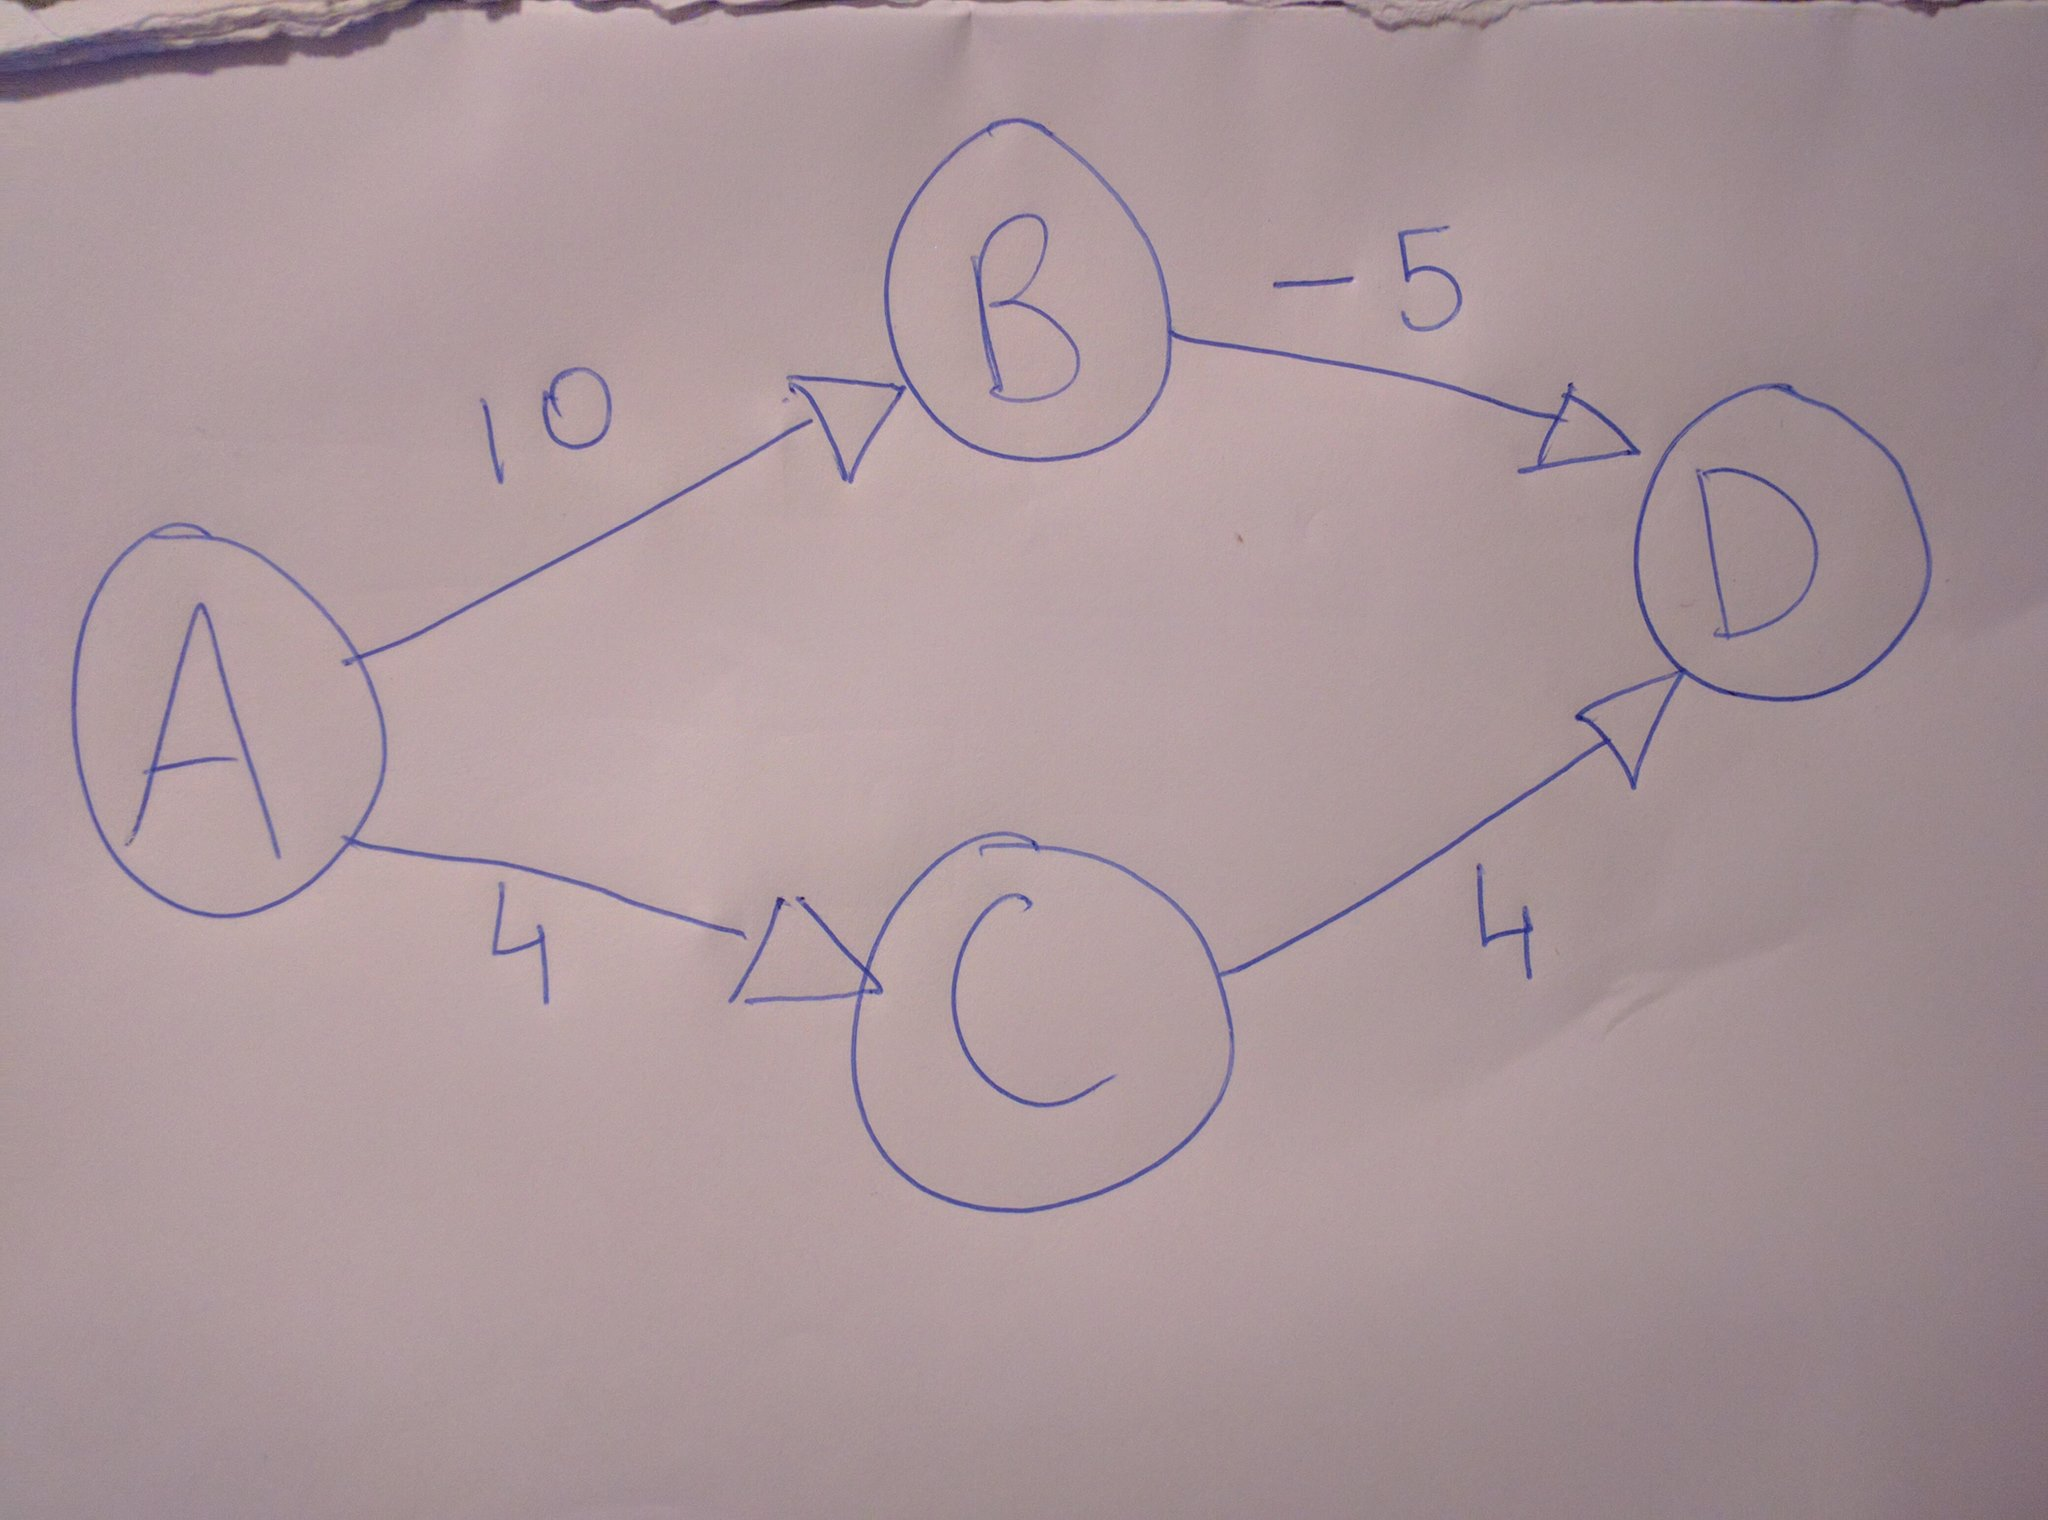
\includegraphics[scale=0.1]{fig_negativeweights}
~\\~\\

\section{A*}

A* is nearly identical to Dijkstra's, but when a triple $\kwa{<node, from, costSoFar>}$ is put into the fringe, an extra estimate of how long it will take to get from $\kwa{from}$ to $\kwa{dest}$ is added to $\kwa{costSoFar}$. This ``guess'' is called a heuristic. $\kwa{heuristic(n)}$ is the estimate of how long it takes to get to $\kwa{dest}$ from $\kwa{n}$. Pseudocode for A* is identical to Dijkstra's, except for the line where triples are put into the queue.

\begin{lstlisting}
A*(src, dest) {
   pq = $\varnothing$, visited = $\varnothing$
   pq.offer(<src, null, 0>)
   while (pq $\neq$ $\varnothing$) {
      <node, from, costSoFar> = pq.pop()
      if (node == dest) return the path
      if (node $\in$ visited) continue
      visited.add(node)
      for (neigh : node.neighbours()) {
         pq.offer(<neigh, node,  costSoFar + weight(node, neigh) + h(neigh)>)
      }
   }
   return null
}
\end{lstlisting}

\noindent
To illustrate why the heuristic is useful, consider the following example. The value inside the node is the heuristic associated with it. If you run A* on the graph, only paths along the left-hand, shortest path will be visited. if you run Dijkstra's, it will snake back and forth between the two paths. With a good heuristic, you can find the shortest path much faster by only considering the best-looking candidate paths that get you closer to the goal.


~\\~\\
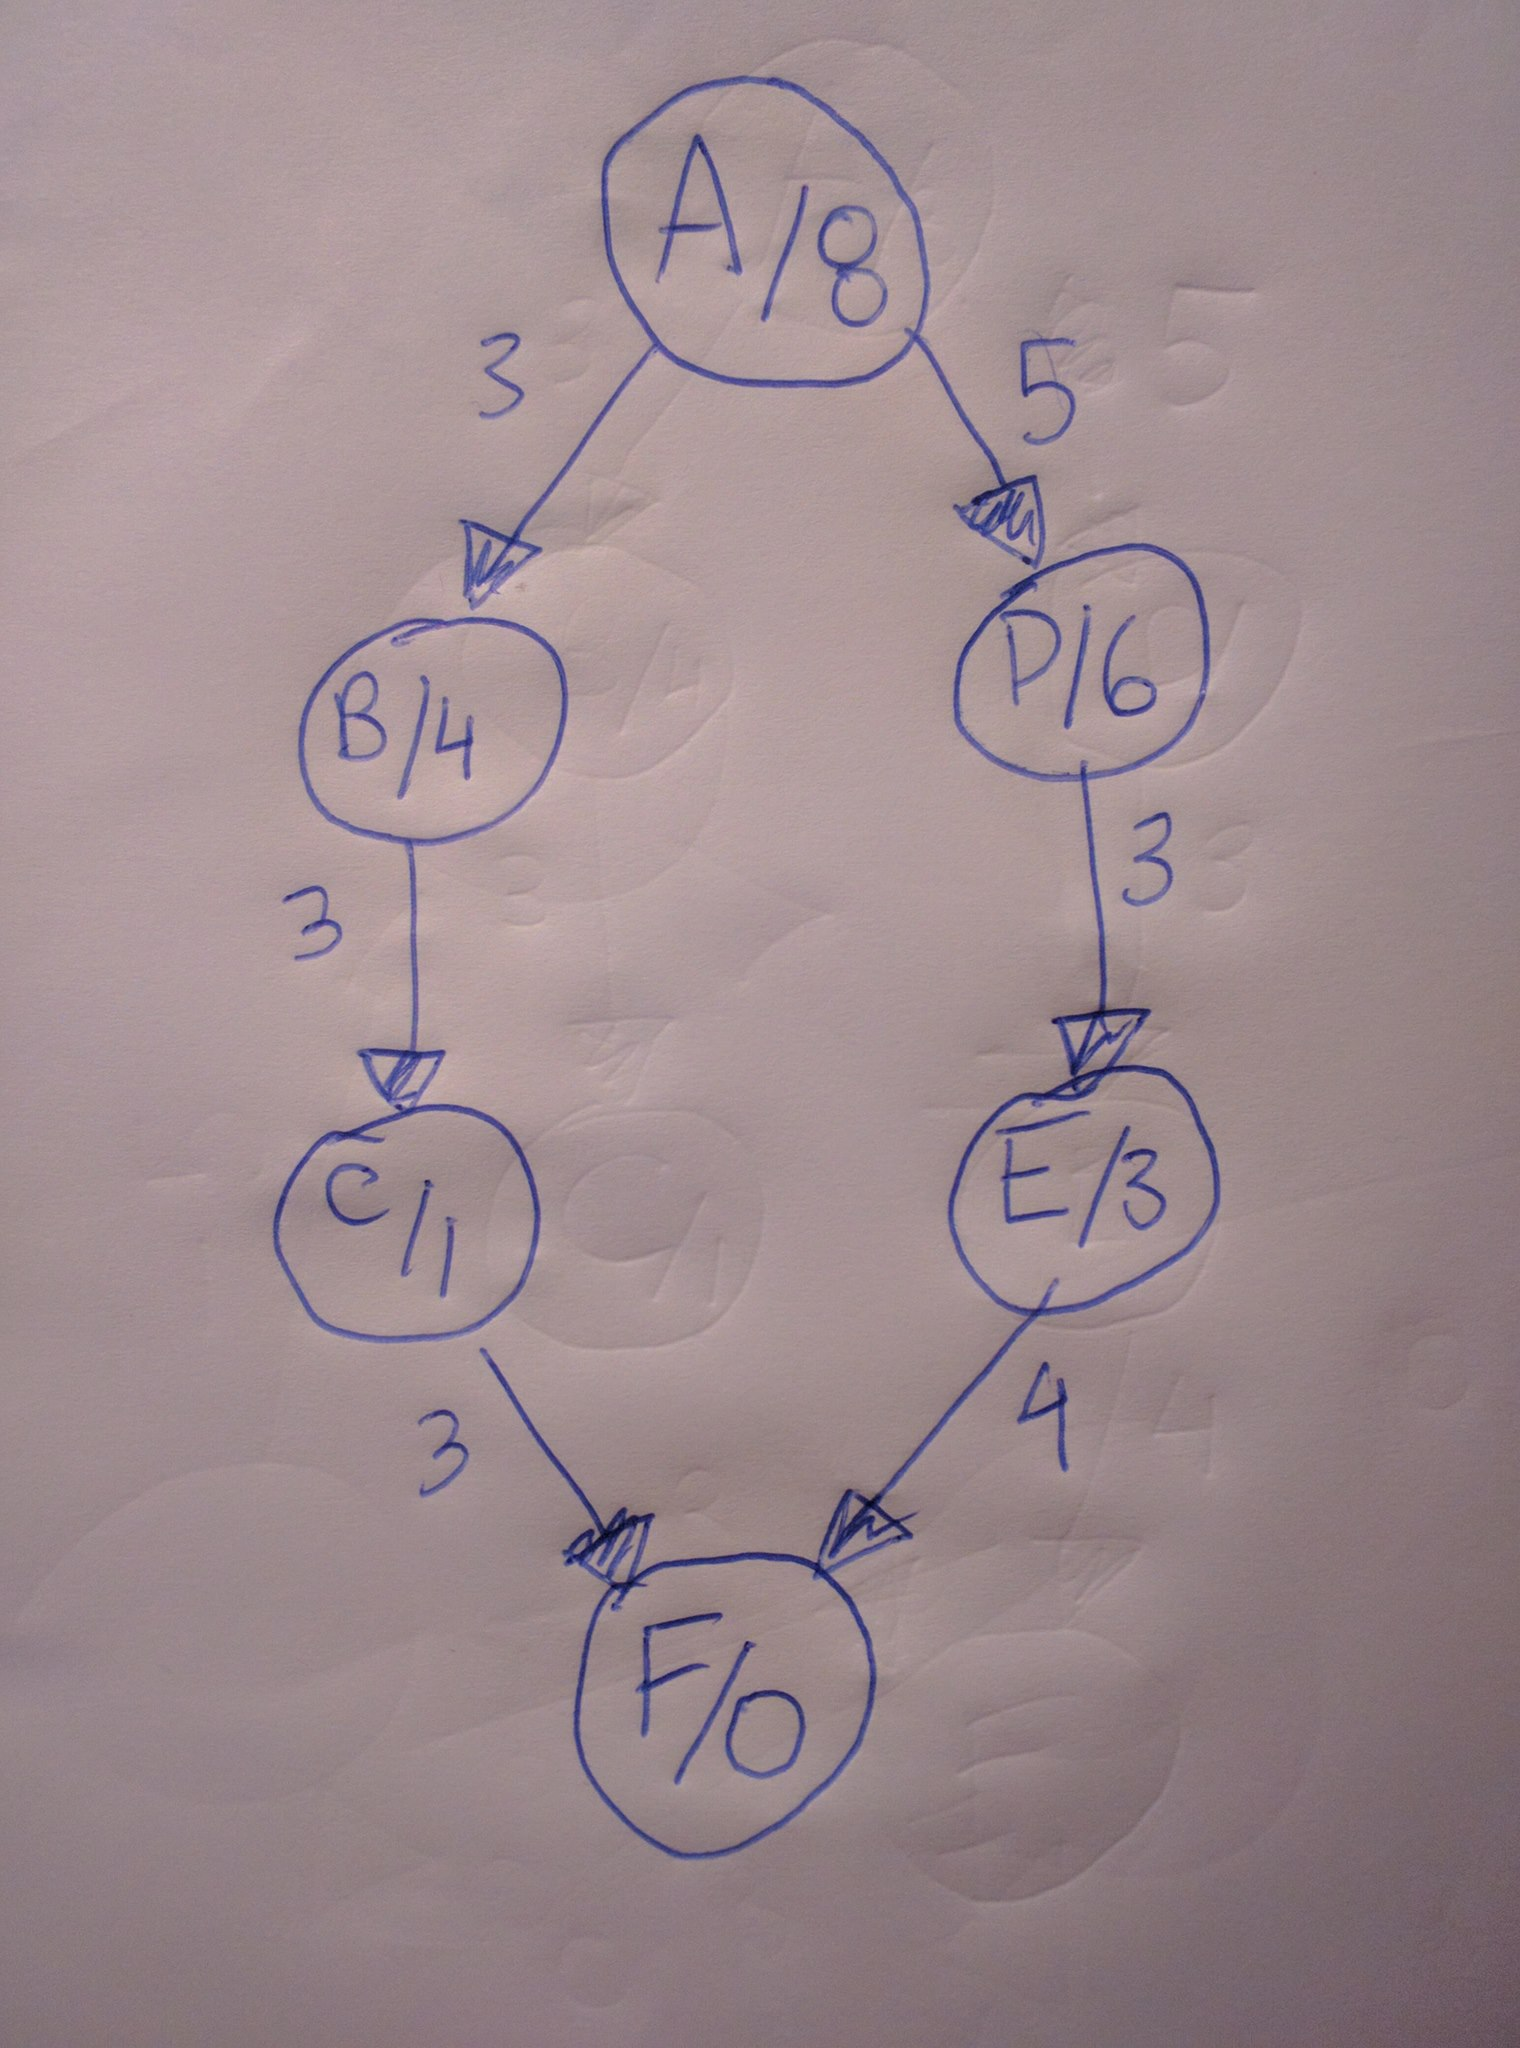
\includegraphics[scale=0.1]{fig_astar}
~\\~\\

\section{Heuristics}

A* works so long as the following two conditions are met:
\begin{enumerate}
	\item Admissible: the heuristic $\kwa{heuristic(n)}$ always underestimates the actual shortest distance from $\kwa{n}$ to $\kwa{dest}$.
	\item Consistent: for any node $\kwa{n}$ and neighbour $\kwa{m}$, $\kwa{heuristic(n) \leq weight(n, m) + heuristic(m)}$.
\end{enumerate}

\noindent
An intuitive reading of a consistent heuristic is that it always guesses smaller as you actually get closer to $\kwa{dest}$.

If a heuristic is not admissible, you may not find the shortest path because a heuristic which wildly overestimates the remaining distance on a node can prevent you ever visiting it --- even if it turns out the estimate was wrong and that direction contained the shortest path. Consider the following example: A $\rightarrow$ C $\rightarrow$ D is the shortest path, but it never gets visited because $\kwa{heuristic(C)}$ makes it look unappealing.

~\\~\\
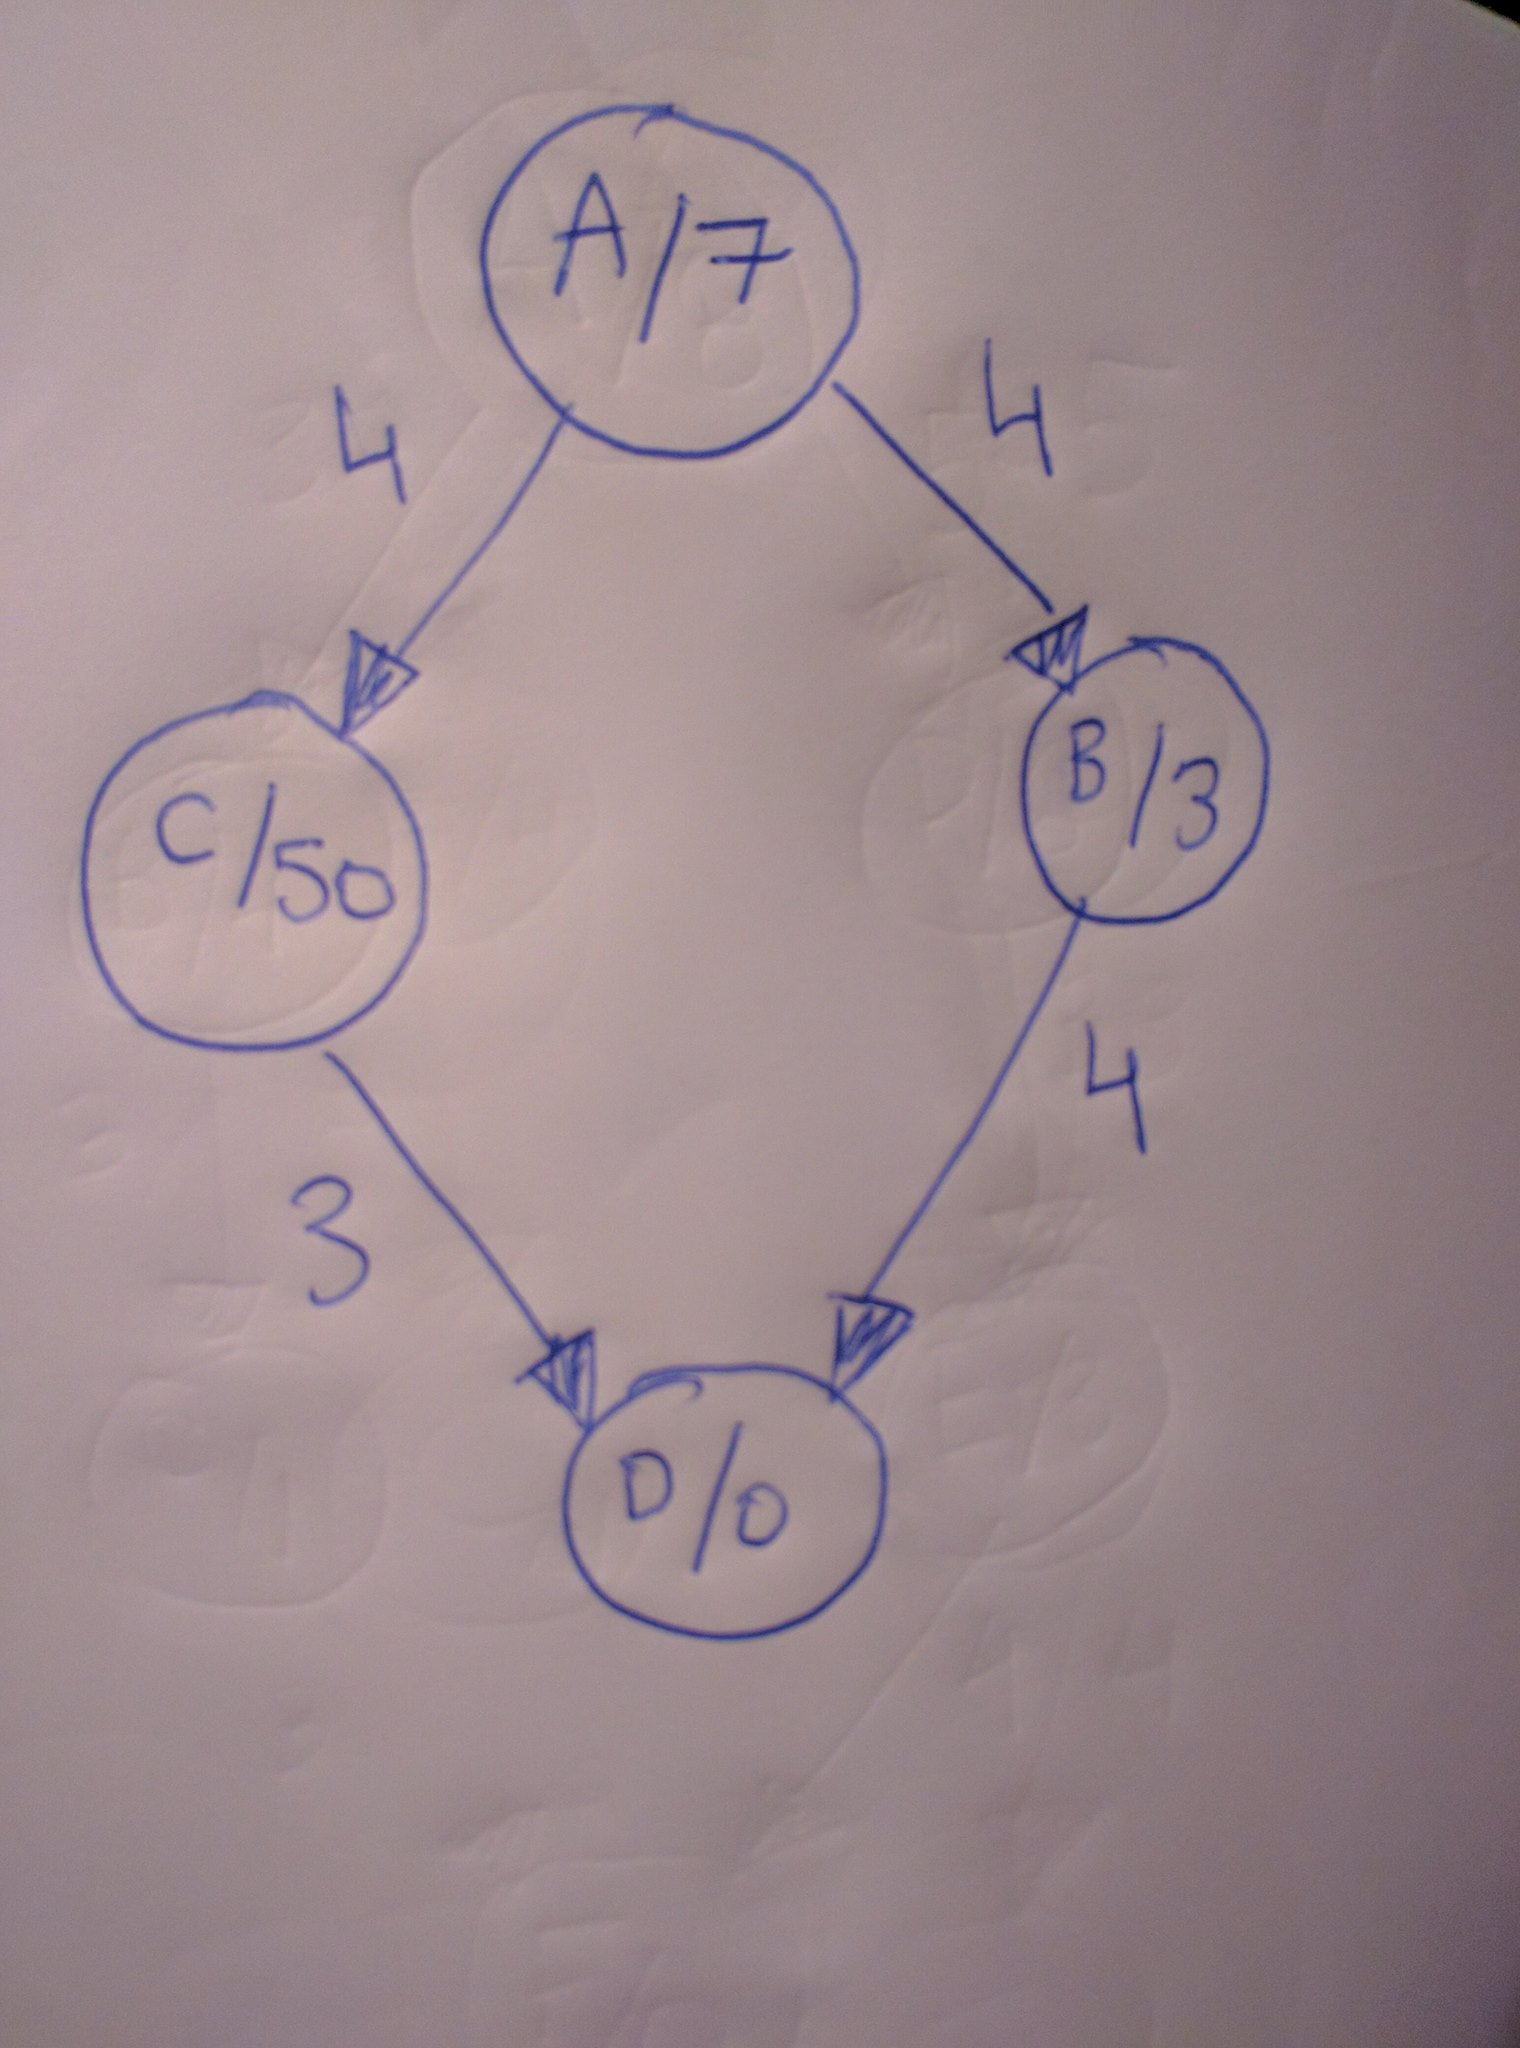
\includegraphics[scale=0.1]{fig_inadmissible}
~\\~\\

\noindent
A* can sometimes work if a heuristic is not admissible. For instance, if the heuristic gives as its guess twice the real length of the shortest path, this will be an inadmissible heuristic (because you are overestimating) but it will still find the shortest path (because you are ``consistently'' overestimating).

Every consistent heuristic is also admissible. This can be proved by induction. Take any node $\kwa{v_1}$ and consider the shortest path from $\kwa{v_1}$ to $\kwa{v_n}$: $\kwa{v_1 \rightarrow v_2 \rightarrow ... v_{n-1} \rightarrow v_n}$. The heuristic $\kwa{h}$ is consistent, so we know $\kwa{h(v_1) \leq w(v_1, v_2) + h(v_2)}$. We can repeat this again for $\kwa{h(v_2)}$, giving the inequality $\kwa{h(v_1) \leq w(v_1, v_2) + w(v_2, v_3) + h(v_3)}$. This process can be repeated until we do it for $\kwa{h(v_n)}$, at which point we have the inequality $\kwa{h(v_1) \leq w(v_1, v_2) + ... + w(v_{n_1}, v_n)}$, meaning the heuristic on $v_1$ is underestimating the cost of the shortest path $v_1 \rightarrow ... \rightarrow v_n$. $\kwa{v_1}$ was an arbitrary node, so this is true for every node in the graph.

Making a heuristic consistent is enough to ensure the pseudocode for A* given above will work. Straight-line distance is a consistent (and by implication, admissible) heuristic, so it can be used as your heuristic in the assignment.

If a heuristic is not admissible, then it isn't consistent. This follows by the identity $P \implies Q \equiv \neg P \implies \neg Q$. This reformulation may be useful when trying to determine if a heuristic is consistent or not --- if you can show it is not admissible, then it's automatically not consistent.

\section{Cost of Dijkstra's/A*}

If a priority queue has size $S$, it costs $log(S)$ to both add and pop. The number of times we add to the queue, plus the number of times we pop, is going to be the big-oh cost of Dijkstra's and A*. At most, one triple could be added to the queue per edge. This gives $\mathcal{O}(E)$ as a bound for the size of the queue. Popping from the queue happens at most once per element of the queue, so the cost of popping is $\mathcal{O}(E \cdot log (E))$. 

The number of times the inner loop gets executed will be the number of times we add to the queue. We've already argued this is $\mathcal{O}(E)$, but another reason to see why is that the loop on line 9 is executed once per node in the graph (since each node is processed at most once). The number of times around the loop is the number of outgoing edges of the particular node we're visiting. In a directed graph, each edge appears in exactly one node's outgoing set. Therefore, the sum of the number of outgoing edges on every node is the same as the number of edges in the graph --- $\mathcal{O}(E)$. By whatever reasoning, the number of times we add to the priority queue is $\mathcal{O}(E \cdot log(E))$.

Together this gives a big-oh cost of $\mathcal{O}(E \cdot log(E) + E \cdot log(E) = \mathcal{O}(E \cdot log(E))$. Some online sources will report a different big-oh cost --- the precise cost will depend on what underlying data structure is used (in our case, a priority queue) and which version of A*/Dijkstra's (there are several slightly different ways to implement it).


\section{Articulation Points}

We call a node an articulation point if deleting it from a graph would increase the number of components. For the assignment, we're only interested in undirected graphs. In particular, for our application of this algorithm, we want to treat directed edges as being undirected (one-way road rules are not important in emergency situations). If you run the algorithm in this section, obeying one-way rules, it would highlight a slightly different kind of articulation point (a node whose removal breaks strong connectivity). The example below highlights some articulation points.

~\\~\\
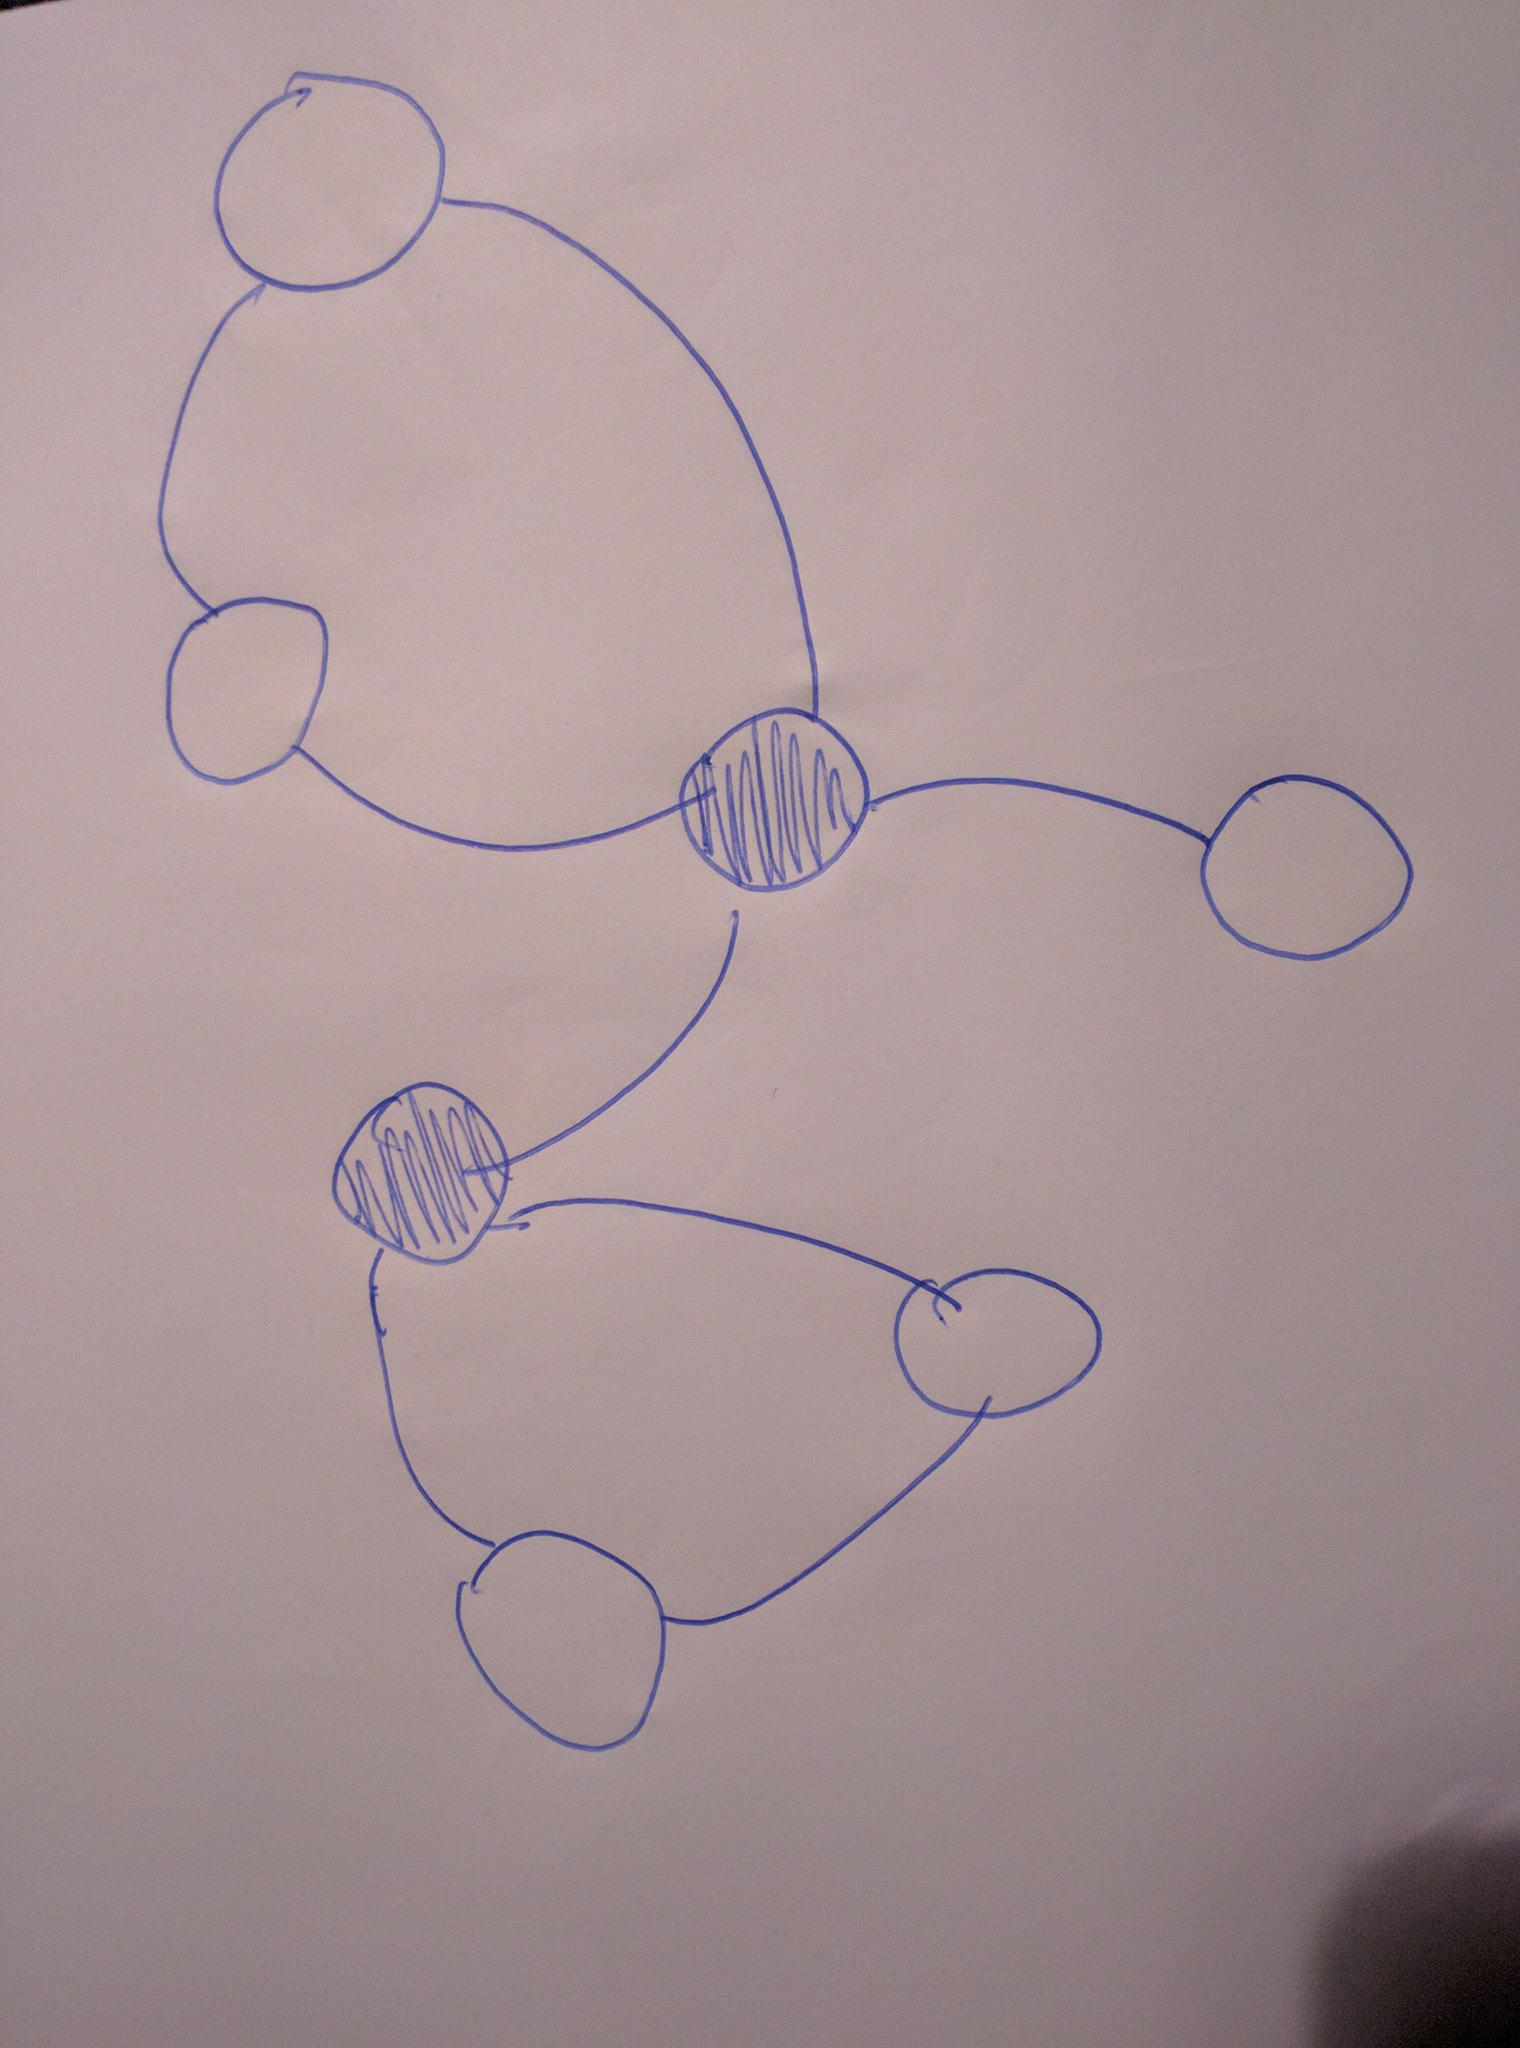
\includegraphics[scale=0.1]{fig_artpts}
~\\~\\


\noindent
The algorithm for finding articulation points is based on depth-first search. The idea is as follows. Each level of recursion is assigned a depth. To determine if a node $\kwa{n}$ at depth $n$ is an articulation point, we look at the children below it, i.e. the ones we have yet to recurse to, and see if any of them can reach back up to an earlier depth. If this can be done, disconnecting $\kwa{n}$ will not disconnect its children (because they have a path back up to an earlier depth); if it can be done, disconnceting $\kwa{n}$ will disconnect its children (because there is no path back up to an earlier depth than the one through $\kwa{n}$). Here is the pseudocode.

\begin{lstlisting}
artPtsFromRoot(root) {
   root.count = 0, numSubtrees = 0, artPts = $\varnothing$
   for (neigh $\in$ root.neighbours()) {
      if (neigh.count = $\infty$) {
         artPts(neigh, 1, root)
         numSubtrees++
      }
   }
   if (numSubtrees > 1) {
      artPts.add(root)
   }
}
\end{lstlisting}

\begin{lstlisting}
artPts(node, count, from) {
   node.count = count, reachback = count
   for (neigh $\in$ node.neighbours()) {
      if (neigh == parent) {
         continue
      }
      else if (neigh.count < $\infty$) {
         reachback = min(neigh.count, reachback)
      else {
         childreach = artPts(neigh, count+1, node)
         if (childreach $\geq$ node.count) {
            artPts.add(node)
         }
         reachback = min(childreach, reachback)
      }
   }
}
\end{lstlisting}

There are two versions of the algorithm. One is for the root node --- the point at which the depth-first search begins. This version initialises the algorithm and recursively computes the articulation points on all nodes neighbouring the root node. If you have to make more than one recursive call, it means that neighbours of $\kwa{root}$ were unable to visit each other except through the path from $\kwa{root}$ --- then disconnecting $\kwa{root}$ woudl disconnect them, and therefore it is an articulation point. This is the reason why $\kwa{numSubtrees}$ is tracked.

The recursive version first sets the count (depth) of a node. Its reachback is initially the same as its count (depth), because any node can reachback to at least itself. For every neighbour of the node (excepting the one we just came from --- this is checked on line 4), it either has been visited or it hasn't. If it has been visited --- and it has been assigned a count (line 7) --- then $\kwa{node}$ can reach to at least that neighbour's depth, so we should update it if it is the lowest depth we've reached so far. Otherwise, the neighbour hasn't been visited, so we recursively compute articulation points from that neighbour and figure out how far back up the graph it can reach (line 10). If the child's reach is no less than the depth of the node we're currently at (line 11), that makes us an articulation point (the only way to get back up to the part of the graph we came from is via $\kwa{node}$). 


\section{Implementing Articulation Points}

I would say there are two main ways to implement articulation points. One way is to add a field to your $\kwa{Node}$ class called $\kwa{count}$, like so:

\begin{lstlisting}
public class Node {
   private int count;
   // ... other stuff here
}
\end{lstlisting}

\noindent
In your articulation points algorithm, you will have to reset the $\kwa{count}$ field of every node before running the algorithm. Another approach is to store a map telling you what is the count of every node. This map could either be stored as a field (and reset every time you call the algorithm), or passed as an argument to $\kwa{artPts}$.

\begin{lstlisting}
public class ArtPts {
   private Map<Node, Integer> countMap;
   private Set<Node> artPts;
   
   ...
   
}
\end{lstlisting}

\begin{lstlisting}
public class ArtPts {

   public Set<Node> artPtsFromRoot(Node root) { ... }

   public int artPts(Node node, Node from,
                       Map<Node, Integer> countMap, Set<Node> artPts) {
      ...
   }
}

\end{lstlisting}

\noindent
Note that calling $\kwa{artPtsFromRoot}$ will only find articulation points in one component of the graph (the one containing the root node). To find articulation points across all components, you will need to call $\kwa{artPtsFromRoot}$ with a node from every component. To do this, you can iterate over all nodes in the graph, calling $\kwa{artPtsFromRoot}$ so long as they haven't been visited. This will require another wrapper method. You will have to leave $\kwa{node.count}$ with its value between calls to $\kwa{artPtsFromRoot}$. If doing it with maps, you will need to remember the $\kwa{countMap}$ generated by each call to $\kwa{artPtsFromRoot}$. 

\section{Cost of Articulation Points}

Each node is visited exactly once, so $\kwa{artPts}$ is called once per node in the graph. In $\kwa{artPts}$, we do some constant number $c$ of operations, and a number of operations proportional to the number of neighbours of this node. The call to node $\kwa{v_i}$ therefore has cost $\kwa{c + |v_i.neighbours|}$. $\kwa{artPts}$ is called $\mathcal{O}(N)$ times, so the number of constant operations is $\mathcal{O}(N \cdot c) = \mathcal{O}(N)$. The number of operations performed by the loop is $|v_1.neighbours| + |v_2.neighbours| + ... + |v_n.neighbours|$. In an undirected graph, each edge is in the neighbours of two nodes (the two nodes being those on either side of the edge). Therefore, the sum of the sizes of all the neighbours of all the nodes in the graph is going to be $2 \cdot N = \mathcal{O}(E)$. The total cost is therefore $\mathcal{O}(N+E)$.

\end{document}






